\documentclass[12pt]{article}

\usepackage{xeCJK}
\usepackage{sectsty}
\usepackage{amsmath}
\usepackage{amsfonts}
\usepackage{graphicx}
\usepackage{amsmath}

\DeclareGraphicsExtensions{.png,.pdf}

\setCJKmainfont{AozoraMinchoRegular.ttf}

\title{離散構造}
\date{}

\sectionfont{\fontsize{12}{15}\selectfont}

\newcommand\floor[1]{\lfloor#1\rfloor}

\newcommand{\problem}{%
  \refstepcounter{section}%
  \section*{問 \thesection}}
 
\begin{document}

\maketitle

\problem\label{Chapter 3 - Answer}

\begin{flushleft}
(1-a) グラフ \( G \) は以下の通り. 冬の大三角である.

\begin{center}
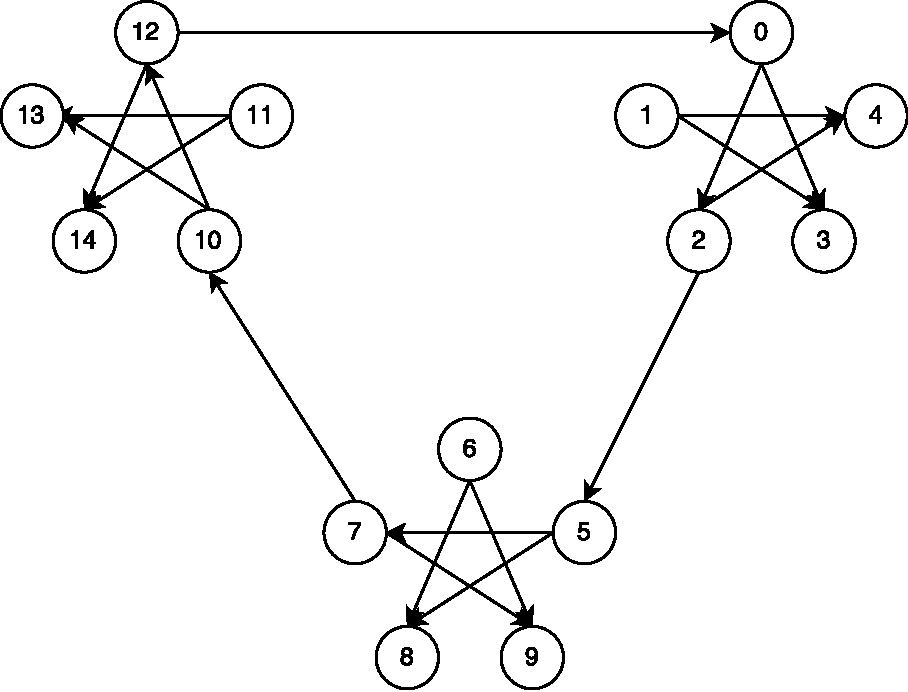
\includegraphics[scale=0.5]{graph}
\end{center}

(1-b) 頂点の数は 15, 辺の数は 18 である. \\

(1-c) 

\begin{center}
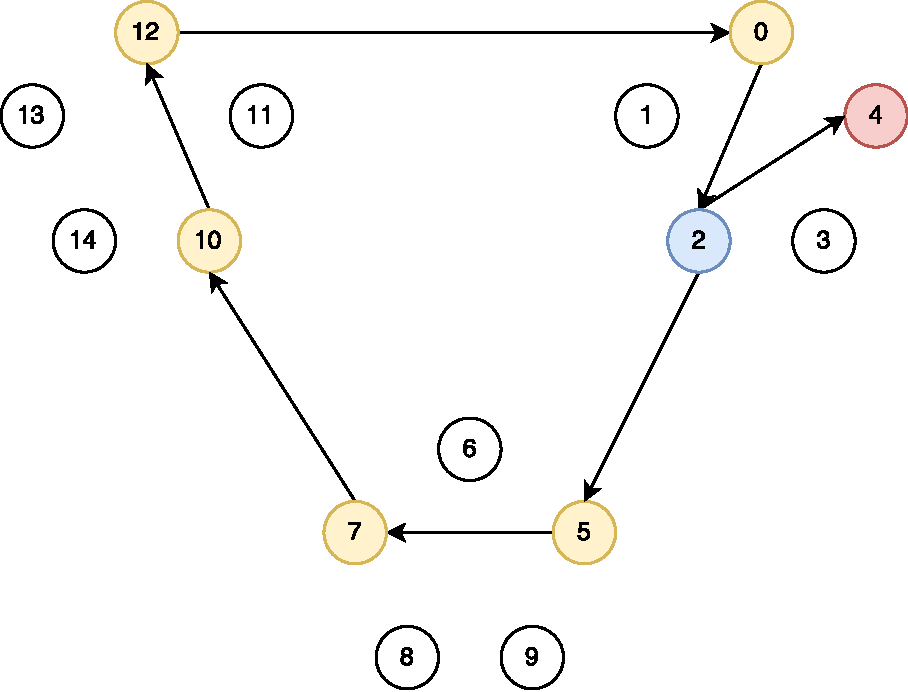
\includegraphics[scale=0.5]{graph_ans2}
\end{center}

最長の単純道は

\[ \langle 2, 5, 7, 10, 12, 0, 2, 4 \rangle \]

であり, その長さは 7 である. \\

\vspace{5mm}

(1-d) 2項関係 $S \circ $S を辺として持つグラフを \( G' \) とする.
\begin{itemize}
    \item 有向グラフ \( G' \) の任意 \( x \) について \( \forall x (xRx) \) でないため, 反射的でない.
    \item \( \forall xy(xRy \Rightarrow yRx \) でないため, 対称的でない.
    \item \( \forall xyz(xRy \wedge yRz \Rightarrow xRz) \) でないため, 推移的でない.
\end{itemize}
よって, 同値関係でない.
\end{flushleft}

(2-a)

\begin{itemize}
    \item Base Case: \( \langle \rangle \in S \)
    \item Base Case: 任意の \( x \in D \) について, \( \langle x \rangle \in S \)
    \item Induction Step: \( L \in S \wedge x \in D \wedge x mod 3 = 0 \vee x mod 5 = 0 \Rightarrow cons(x, L) \in S \)
\end{itemize}

(2-b)

\begin{equation}
\begin{split}
length(\langle 1, 0, 1, 1 \rangle) & = 1 + length(\langle 0, 1, 1 \rangle) \\
                                   & = 1 + (1 + length(\langle 1, 1 \rangle)) \\
                                   & = 1 + (1 + (1 + length(\langle 1 \rangle)) \\
                                   & = 1 + (1 + (1 + (1 + \langle \langle))) \\
                                   & = 1 + (1 + (1 + (1 + 0))) \\
                                   & = 4
\end{split}
\end{equation}

\begin{equation}
\begin{split}
    calc(\langle 1, 0, 1, 1 \rangle, length(\langle 1, 0, 1, 1 \rangle))
    & = calc(\langle 1, 0, 1, 1 \rangle, 4) \\
    & = calc(\langle 0, 1, 1 \rangle, 3) + 1 \cdot 2^3 \\
    & = (calc(\langle 1, 1 \rangle, 2) + 0 \cdot 2^2)  + 1 \cdot 2^3 \\
    & = ((calc(\langle 1 \rangle, 1) + 1 \cdot 2^1) + 0 \cdot 2^2)  + 1 \cdot 2^3 \\
    & = (((calc(\langle \rangle, 0) + 1 \cdot 2^0) + 1 \cdot 2^1) + 0 \cdot 2^2)  + 1 \cdot 2^3 \\
    & = (((0 + 1 \cdot 2^0) + 1 \cdot 2^1) + 0 \cdot 2^2)  + 1 \cdot 2^3 \\
    & = 11
\end{split}
\end{equation}

(2-c)
\begin{equation}
\begin{split}
    comp(\langle 0, 1, 0, 0 \rangle, \langle 0, 1, 1, 0 \rangle)
    &= Fcomp(\langle 1, 0, 0 \rangle, \langle 1, 1, 0 \rangle) \\
    &= F(Tcomp(\langle 0, 0 \rangle, \langle 1, 0 \rangle)) \\
    &= F(T(Fcomp(\langle 0 \rangle, \langle 0 \rangle))) \\
    &= F(T(F(Fcomp(\langle \rangle, \langle \rangle)))) \\
    &= FTFF
\end{split}
\end{equation}

(2-d)
\begin{itemize}
    \item Base Case (\( L_1 = nil \wedge L_2 = nil \) のとき): \\
    左辺において, \( length \) の定義より, \( l = length(\langle \rangle) = 0 \). また, \( calc \) の定義より \( calc(\langle \rangle, 0) = 0\). \\
    右辺において, \( comp \) と \( serialize \) の定義より \( calc(serialize(comp(\langle \rangle, \langle \rangle)), 0) = calc(serialize(\Lambda)) = calc(\langle \rangle) = 0 \) となり, (左辺) = (右辺) より, 成立.
    \item Induction Step (\( n = 0 \wedge L_1 = cons(n, L_1') \wedge L_2 = cons(n, L_2') \wedge l > 0 \) のとき):
    左辺において, \( calc \) の定義より, \\
    \( calc(cons(n, L_1'), l) = calc(L', l - 1) + n \cdot 2^{l - 1} \) \\
    \( calc(cons(n, L_1'), l) = calc(L', l - 1) + 0 \cdot 2^{l - 1} \).
    右辺において, \( comp \) と \( serialize \) の定義より \\
    \( calc(serialize(comp(cons(n_1, L_1'), cons(n_2, L_2'))), l) \) \\
    \( = calc(serialize(Fcomp(L_1', L_2')), l) \) \\
    \( = calc(cons(0, serialize(comp(L_1', L_2'))), l) \) \\
    \( = cons(n, calc(serialize(comp(L_1', L_2')), l))  \) \\
    \( = calc(serialize(comp(L_1', L_2')), l - 1) + n \cdot 2^{l - 1} \) \\
    \( = calc(serialize(comp(L_1', L_2')), l - 1) + 0 \cdot 2^{l - 1} \).
    ここで, 帰納法の仮定より, \( calc(L_1', l) = calc(serialize(comp(L_1', L_2')), l) \) であるから, \( calc(L_1, l) = calc(serialize(comp(L_1, L_2)), l) \) が成立.
    \item Induction Step (\( n = 1 \wedge L_1 = cons(n, L_1') \wedge L_2 = cons(n, L_2') \wedge l > 0 \) のとき):
    左辺において, \( calc \) の定義より, \\
    \( calc(cons(n, L_1'), l) = calc(L', l - 1) + n \cdot 2^{l - 1} \) \\
    \( calc(cons(n, L_1'), l) = calc(L', l - 1) + 1 \cdot 2^{l - 1} \).
    右辺において, \( comp \) と \( serialize \) の定義より \\
    \( calc(serialize(comp(cons(n_1, L_1'), cons(n_2, L_2'))), l) \) \\
    \( = calc(serialize(Tcomp(L_1', L_2')), l) \) \\
    \( = calc(cons(1, serialize(comp(L_1', L_2'))), l) \) \\
    \( = cons(n, calc(serialize(comp(L_1', L_2')), l))  \) \\
    \( = calc(serialize(comp(L_1', L_2')), l - 1) + n \cdot 2^{l - 1} \) \\
    \( = calc(serialize(comp(L_1', L_2')), l - 1) + 1 \cdot 2^{l - 1} \).
    ここで, 帰納法の仮定より, \( calc(L_1', l) = calc(serialize(comp(L_1', L_2')), l) \) であるから, \( calc(L_1, l) = calc(serialize(comp(L_1, L_2)), l) \) が成立.\\
    よって, \( List_D \) の任意の要素 \( L_1, L_2 \) について, \( L_1 \) と \( L_2 \) の各要素が全て同じとき, \( calc(L_1, l) = calc(serialize(comp(L_1, L_2)), l) \) が示される.
\end{itemize}

\end{document}